% Full instructions available at:
% https://github.com/elauksap/focus-beamertheme

\documentclass{beamer}
\usetheme{focus}


\title{Enzymbasierte digitale Biosensoren f{\"u}r medizinische Anwendungen}
%\subtitle{Biosensoren in Kombination mit Biocomputing}
\author{Maren Krafft}
%\titlegraphic{
\includegraphics[scale=1.25]{focuslogo.pdf}}
\institute{Universit{\"A}t Passau \\ Lehrstuhl f{\"u}r technische Informatik}
\date{02 08 2018}

\AtBeginSubsection[]
{
	\begin{frame}<beamer>{Gliederung}
	\tableofcontents[currentsection,currentsubsection]
	\end{frame}
}
\begin{document}
    \begin{frame}
        \maketitle
    \end{frame}

	\begin{frame}{Motivation}
		\begin{itemize}
			\item Bietet neue M{\"o}glichkeiten in der medizinischen Anwendung
			\item (R)evolution des herk{\"o}mmlichen Biosensors
			\item Mehrere Inputs k{\"o}nnen direkt verarbeitet werden
			\item Beispiele: 
			\begin{itemize}
				\item "Feedback Loops"
				\item Sense-Act-Treat Device
				\item Personalisierte Medikation
				\item Schnelle Reaktion in Notf{\"a}llen
			\end{itemize}
		\end{itemize}
	\end{frame}
   
    \begin{frame}{Gliederung}
    \tableofcontents
    % You might wish to add the option [pausesections]
	\end{frame}

	\section{Begriffserkl{\"a}rung}
	\begin{frame}{Wichtige Begriffe}
		\begin{itemize}
			\item Enzym = organische Verbindung
			\item Biosensor = Komplex zur biochemischen Analyse von Stoffen
			\item Trauma = Sch{\"a}digung, Verletzung oder Verwundung lebenden Gewebes
			\item H{\"a}morrhagischer Schock = Minderdurchblutung
			\item Substrat = Stoff, der durch ein Enzym umgesetzt
		\end{itemize}		
	\end{frame}
 
 	\section{Konzept}
 	
 	\subsubsection{Biosensoren}
 	
 	\begin{frame}<beamer>{Gliederung}
 	\tableofcontents[currentsection,currentsubsection]
 	\end{frame}
 	
    \begin{frame}{Biosensoren}
       Aufbau: 
        \begin{figure}[H] \centering 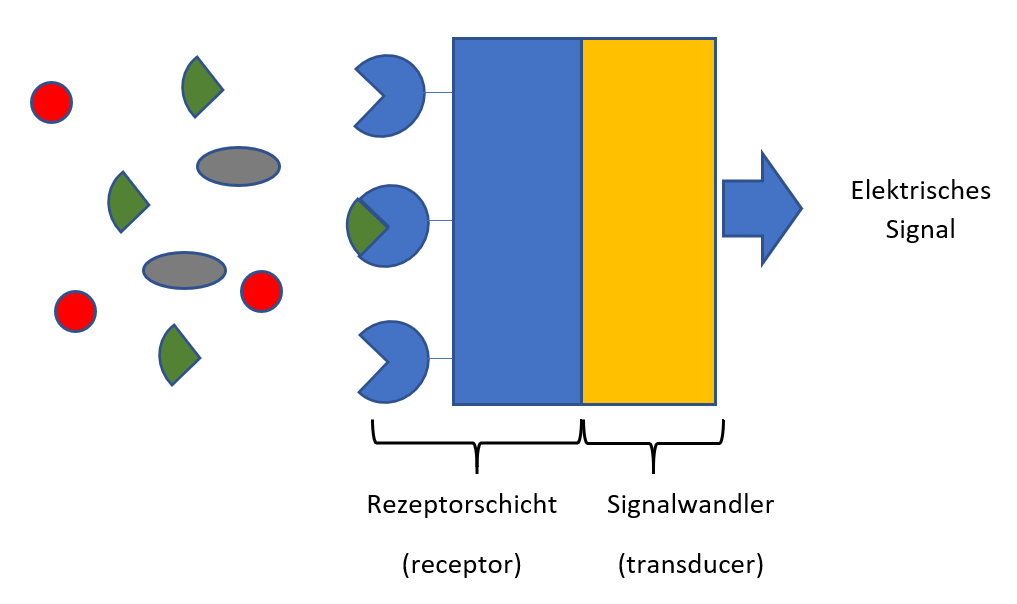
\includegraphics[scale= 0.33]{pics/biosensor.png} \caption{Eigene Darstellung} \label{img:and} 	
       \end{figure}
    \end{frame}



	\subsubsection{Enzymbasierte Logikgatter}
	
	\begin{frame}<beamer>{Gliederung}
	\tableofcontents[currentsection,currentsubsection]
	\end{frame}

    \begin{frame}{Enzymbasierte Logikgatter}
    Umsetzung von aus der Informatik bekannten Logikgattern mit biochemische Substanzen
    
    	\begin{itemize}	
    		\item Enzyme als Logik
    		\item Zwei oder mehr biochemische Substanzen als Input
    		\item Reaktion mit dem Enzym produziert eine weitere biochemische Substanz
    		\item Konzentration einer bestimmten biochemischen Substanz gr{\"o}\ss{}er/kleiner als kritischer Wert entspricht den Booleanwerten 1 und 0
    	\end{itemize}     
    \end{frame}
        
    \begin{frame}{Enzymbasierte Logikgatter - Beispiel 'AND'}
    
    Enzyme: Gox = Glucose-Oxidase und Cat = Katalase\\
    Inputs: Glucose und H\textsubscript{2}O\textsubscript{2}
    
     \begin{figure}[H] \centering 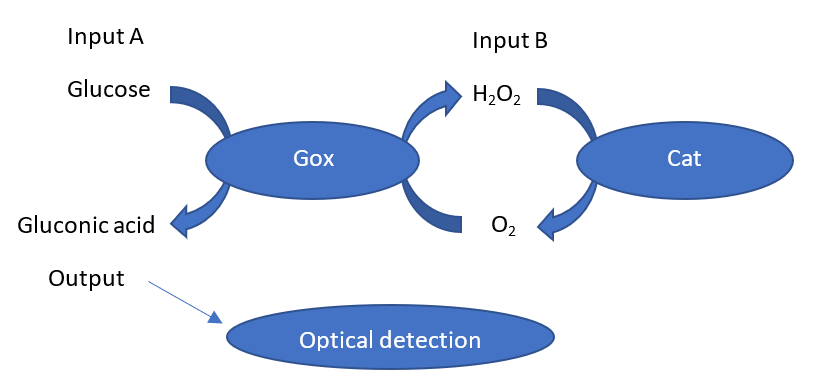
\includegraphics[scale= 0.33]{pics/ANDneu.png} \caption{Eigene Darstellung nach \cite{hallo4} } \label{img:and} 	
   	 \end{figure}
  
    \end{frame}


    \subsubsection{Enzymbasierte Biosensoren}
    
    \begin{frame}<beamer>{Gliederung}
    \tableofcontents[currentsection,currentsubsection]
	\end{frame}
    
    \begin{frame}{Netzwerke aus enzymbasierten Logikgattern}
    	Durch Kombination mehrerer enzymbasierter Logikgatter ist es m{\"o}glich ein Netzwerk zu erschaffen.
    	
    	Beispiel: 
    	\begin{itemize}
    		\item Enzyme: ADH (Alkoholhydrogenase), GDH (Glucose-Dehydrogenase), GOX (Glucose-Oxidase)
    	\end{itemize}
    	\begin{figure}
    		\centering \scriptsize 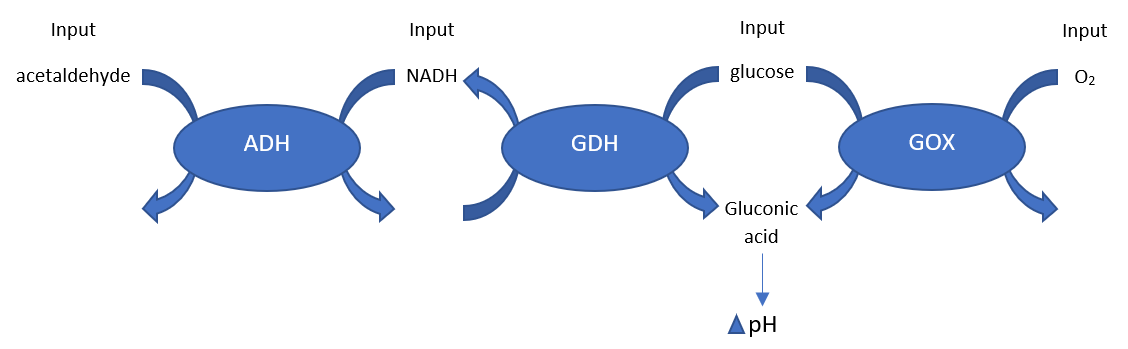
\includegraphics[scale= 0.30]{pics/network1.png}
    	\caption{Eigene Darstellung nach \cite{hallo4}} 
   		\end{figure}
   		
   	
    
	\end{frame}

	\begin{frame}{Netzwerke aus enzymbasierten Logikgattern}
	
	\begin{figure}
		\centering \scriptsize 
		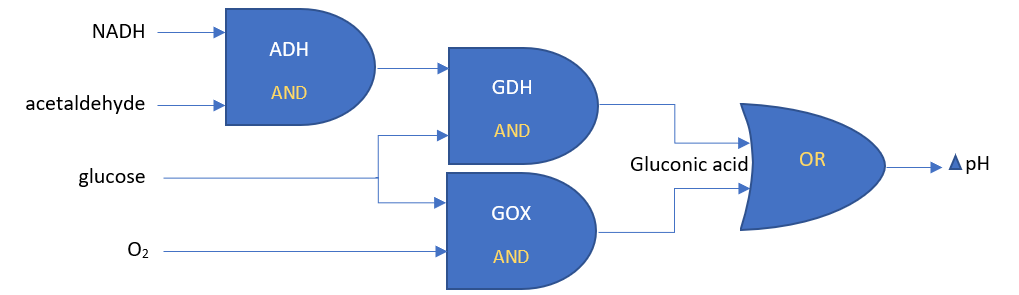
\includegraphics[scale = 0.30]{pics/network2.png} \caption{Eigene Darstellung nach \cite{hallo4}} 
	\end{figure}

	
	\end{frame}


	\begin{frame}{Kombination mit einem Signalwandler}
	
		Durch Hinzuf{\"u}gen eines Signalwandlers (Transducer) zu einem Netzwerk ist es m{\"o}glich, einen Biosensor zu erschaffen, der mehrere Inputs erh{\"a}lt und ein lesbares Signal ausgeben kann.\\
		
		
        \begin{figure}[H] \centering \includegraphics[scale= 0.30]{pics/pH.png} \caption{Eigene Darstellung nach \cite{hallo4}} \label{img:ph} 
        \end{figure}
        
    \end{frame}
 
 
 %für medizinische anwendungen   
   	\begin{frame}{Gliederung}
   	\tableofcontents
	\end{frame}



   	\section{Medizinische Anwendungen}
   		\begin{frame}{Design f{\"u}r medizinische Anwendungen}
   			\begin{itemize}
   				\item Verletzungen und Krankheiten werden im K{\"o}rper durch Konzentrationen spezifischer Stoffe angezeigt
 				\item Enzymbasierte Biosensoren sollen diese Stoffe als Inputs verwenden, um R{\"u}ckschl{\"u}sse auf den Gesundheitszustand zu erlauben
   				\item Konzentration gr{\"o}\ss{}er als kritischer Wert = Boolean 1; weniger als kritischer Wert = Boolean 0
   				\item Der Biosensor soll mehrere krankheitsspezifische Konzentrationen zeitgleich analysieren und ein ja/nein Ergebnis ausgeben  
   			\end{itemize}
   		\end{frame}
   
   	\begin{frame}{Beispiel hemorrhagischer Schock}
   			\begin{itemize}
   				\item Enzyme: Glucose-Dehydrogenase, Lactase-Oxidase, Meerrettich-Oxidase
   				\item Inputs: Glucose, Lactase, Norepinephrine
   				\item Outputs: NADH, Norepiquinone
   			\end{itemize}
  		
  
   		\begin{table}
   		\scriptsize
   		\begin{tabular}{l|c|c|c|c|c|}
   		condition & norepiquinone & NADH & glucose & lactate & norepinephrine\\ \hline
   		traumatic brain injury & 1&0&0&1&1\\
   		hemorrhagic shock & 1&1 &1&1&1\\ 
   		\end{tabular}\\
   		\caption{Eigene Darstellung nach \cite{hallo4}}
   		\end{table}
	\end{frame}

  
	\begin{frame}<beamer>{Gliederung}
	\tableofcontents
	\end{frame}





%Überlegungen
   \section{{\"U}berlegungen}
   	
   \begin{frame}{Oberfl{\"a}chenfixierung}   		
   		\begin{itemize}	
   			\item Bisher: Experimente mit L{\"o}sungen in Petrischalen
   			\item Problem: keine Struktur = keine medizinische Anwendung
   			\item Herausforderung: Physische Fixierung und Trennung der einzelnen Reagenzschichten
   			\item Ziel: Vermeidung von Querreaktionen und Kombinierbarkeit   			
   		\end{itemize}
	\end{frame}
	
	
	\begin{frame}{{\"U}bertragungskomplexit{\"a}t}		
		\begin{itemize}	
			\item Bisher: Reagenzschichten und Signalwandler k{\"o}nnen nur wenige Inputs verarbeiten
			\item Problem: Komplexere Netzwerke erfordern leistungsf\"ahigere Reagenzschichten und Signalwandler			
		\end{itemize}
		\end{frame}

	\begin{frame}{Definition der Booleanwerte 1 und 0}		
		\begin{itemize}	
			\item Bisher: H\"aufig willk\"urliche 1 und 0 Booleanwerte ohne medizinische Relevanz 
			\item Herausforderung: 0 als Normalkonzentration und 1 als medizinisch kritischer Wert
			\item Ziel: Experimente und enzymbasierte Biosensoren mit medizinischer Relevanz			
		\end{itemize}
		\end{frame}


	\begin{frame}{Skalierbarkeit}
		\begin{itemize}	
			\item Bisher: Experimente mit sehr spezifischem Ansatz 
			\item Problem: Begrenzte Netzwerkgr\"o\ss{}e; nicht abstrahierbar
			\item Ziel: Kombinierbarkeit von Elementen
		\end{itemize}
	\end{frame}

	\begin{frame}{Wahl relevanter Inputs}		
		\begin{itemize}	
			\item Bisher: Konzepte arbeiten mit medizinisch irrelevanten Stoffen 
			\item Problem: Kein praktischer Nutzen
			\item Ziel: Anwendung des Konzepts auf medizinisch relevante Stoffe
			
		\end{itemize}
	\end{frame}

	\begin{frame}{Medikation}
		\begin{itemize}
			\item Problem: Aktuelle Experimente noch als "Proof Of Concept"
			\item Herausforderung: Entwicklungsreife f\"ur autonome "Sense-Act-Treat" Ger\"ate
		\end{itemize}
	\end{frame}

%Fazit
 	\begin{frame}<beamer>{Gliederung}
 	\tableofcontents
	\end{frame}

   \section{Fazit}
   \begin{frame}{Fazit}
   		\begin{itemize}
   			\item Konzept "steckt noch in den Kinderschuhen"
   			\item Bisher ausschlie\ss{}lich "Proof Of Concept"-Experimente
   			\item Gro\ss{}es Potential f\"ur medizinische Anwendungen
   			\item Zusammenarbeit von Biochemiker, Informatikern und Ingenieuren n\"otig
   			\item Noch viele Entwicklungsschritte notwendig, aber verspricht gro\ss{}artigen Nutzen
   		\end{itemize}
   \end{frame}
   
   
   
%Quellen
	\appendix
	\begin{frame}[allowframebreaks]{Quellen}
	\nocite{*}
	\bibliography{demo_bibliography}
	\bibliographystyle{plain}

	\end{frame}
    
    
\begin{frame}[focus]
Vielen Dank f{\"u}r Ihre Aufmerksamkeit
\end{frame}
   
\end{document}
